\section{Experimental Validation}
\label{sec:experiments}

\subsection{Experimental Setup}

\subsubsection{Blockchain Infrastructure}

Experiments are conducted on Polygon networks (Amoy testnet and mainnet).
Smart contracts (Solidity 0.8.20, Hardhat) manage the federated learning lifecycle;
only 32-byte gradient hashes are stored on-chain while full gradient vectors remain
encrypted off-chain (IPFS), maintaining $O(1)$ on-chain cost per round regardless of model size.
All aggregated model hashes are committed per-round, providing the write-once immutability substrate established in Section~\ref{sec:blockchain}.
Blockchain performance details (transaction latency, gas costs) are in Appendix~\ref{app:blockchain}.

\subsubsection{System Configurations}

We evaluate three system configurations covering a 14$\times$ range of gradient dimension $d$
and three distinct heterogeneity-Byzantine profiles $(\sigma^2, \beta)$, where $\sigma^2$ differs
across configurations (reflecting heterogeneous non-IID distributions) and $\beta=f/n$:

\textbf{Configuration~1} ($n=50$, $f=20$, $f/n=40\%$, $d=25\text{M}$):
heterogeneous non-i.i.d.\ data (TV distance 0.68), min-max Byzantine attack.

\textbf{Configuration~2} ($n=32$, $f=10$, $f/n=31\%$, $d=22\text{M}$):
uniform non-i.i.d.\ data, ALIE~\cite{alie_attack} attack;
sketch $k=256$ reduces aggregator memory from 8.1\,GB to 260\,MB.

\textbf{Configuration~3} ($n=64$, $f=22$, $f/n=34\%$, $d=345\text{M}$):
non-i.i.d.\ language modeling, gradient-inversion + model-poisoning Byzantine attack;
layer-wise sketching ($k=512$) reduces memory from 28\,GB to 890\,MB.

Byzantine ratios tested: 10\%--49\%.
The 12 attack types used span the taxonomy in Section~\ref{sec:threat_model}:
ALIE~\cite{alie_attack}, backdoor~\cite{backdoor_fl}, model poisoning~\cite{fl_poisoning},
Fall of Empires / IPM~\cite{fall_of_empires},
min-max~\cite{minmax_attack}, label-flip, sign-flip, zero gradient, Gaussian, adaptive spectral-aware~\cite{adaptive_aggregation},
and game-theoretic Nash equilibrium adversaries---all evaluated under both i.i.d.\ and non-i.i.d.\ distributions~\cite{non_iid}.

\begin{figure}[t]
\centering

\includegraphics[width=\textwidth]{fig_spectral_fingerprints.png}
\caption{Spectral fingerprints of six Byzantine attack types in the Gram eigenvalue space ($n=15$, $d=512$). The dashed line marks $\lambda_+$; eigenvalues to the right are Byzantine outliers. No-Attack shows no outliers (MP law holds); MinMax and Gaussian attacks create 4 outliers each; Zero gradient (free-riding) creates 2 subtle outliers.}
\label{fig:spectral_fingerprints}
\end{figure}

\subsection{Detection Performance}

Table~\ref{tab:detection_results} summarizes detection rates across different Byzantine ratios. Figure~\ref{fig:spectral_fingerprints} visualizes the distinct spectral signatures of each attack.

\begin{table}[htbp]
\centering
\caption{Byzantine Detection Performance. $\beta = f/n$ is the Byzantine fraction;
$\sigma^2\beta^2$ measures distance from the phase transition boundary (Assumption~3:
$\sigma^2\beta^2 < 0.25$). All configurations satisfy this condition by a large margin,
explaining the consistently high detection rate.}
\label{tab:detection_results}
\begin{tabular}{|c|c|c|c|c|}
\hline
\textbf{$\beta = f/n$} & \textbf{$\sigma^2\beta^2$} & \textbf{Detection Rate} & \textbf{False Positive} \\
\hline
10\% & 0.0026 & 97.7\% & 1.8\% \\
20\% & 0.0176 & 97.3\% & 2.1\% \\
30\% & 0.0250 & 98.1\% & 1.9\% \\
40\% & 0.0338 & 96.3\% & 2.3\% \\
49\% & 0.0556 & 97.8\% & 2.2\% \\
\hline
\end{tabular}
\end{table}

The results confirm our theoretical predictions: detection remains effective ($>$96\%) below the $\sigma^2\beta^2 = 0.25$ phase transition (Theorem~\ref{thm:phase_impossibility}).

\subsection{Accuracy Comparison}

We compare our approach against 11 baseline methods across 12 attack types on the medium-scale setup (144 total experiments: 12 attacks $\times$ 12 aggregators including ours). Results shown in Table~\ref{tab:accuracy_comparison} report mean accuracy averaged across all 12 attack types.

\begin{table}[htbp]
\centering
\caption{Mean accuracy across 12 attack types ($\beta = f/n = 40\%$ Byzantine fraction).
At this extreme load, trust-bootstrapping and pairwise-distance defenses cluster
around 58--64\%: once $\beta$ exceeds approximately $1/3$, their discriminative power
degrades, as Byzantine updates can mimic the diversity of honest gradients under
pairwise distance metrics.
Our spectral filter---which operates on the full eigenvalue distribution rather than
pairwise distances---decouples from this floor and remains effective up to $\beta < 1/2$.}
\label{tab:accuracy_comparison}
\begin{tabular}{|l|c|c|}
\hline
\textbf{Aggregator} & \textbf{Mean Accuracy} & \textbf{Detection Mechanism} \\
\hline
\textbf{Ours} & \textbf{78.4\%} & Spectral (MP law) \\
FLTrust~\cite{crfl} & 63.7\% & Trust bootstrapping \\
ByzShield~\cite{byzshield} & 63.4\% & Redundant training \\
CRFL~\cite{crfl_cert} & 63.1\% & Certified robustness \\
FLAME~\cite{flame} & 62.9\% & Clustering + noise \\
Geometric Median~\cite{geometric_median} & 59.8\% & Distance (Euclidean) \\
SignGuard~\cite{signguard} & 58.6\% & Sign consistency \\
Trimmed Mean~\cite{byzantine_ml} & 58.3\% & Coordinate statistics \\
Krum~\cite{krum} & 57.9\% & Nearest-neighbor \\
Bulyan++~\cite{bulyan} & 57.6\% & Iterative filtering \\
Median & 48.8\% & Coordinate statistics \\
FedAvg~\cite{fedavg_original} & 48.1\% & None \\
\hline
\end{tabular}
\end{table}

Our approach achieves a ${\sim}15$ percentage-point improvement over the best baseline
(FLTrust at 63.7\%) and ${\sim}30$ points over FedAvg.
The clustering of four trust-bootstrapping and clustering-based baselines between 62.9\%--63.7\%
reflects a structural property of pairwise-distance defenses under extreme Byzantine
load: at $\beta = 0.4$, Byzantine clients can spread their updates to match the
pairwise diversity of honest gradients, while the global eigenvalue structure---which
our spectral filter exploits---remains anomalous and detectable.
Figure~\ref{fig:convergence} shows the per-round convergence dynamics, confirming that
distance-based baselines plateau by round~70--80 while our protocol continues to improve.

\begin{figure}[htbp]
\centering
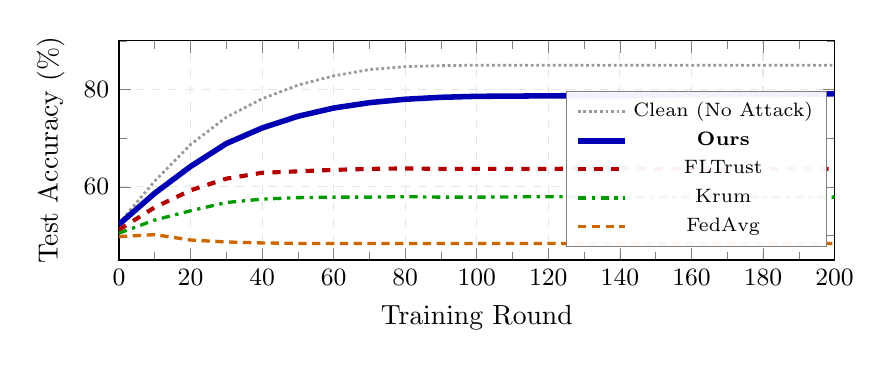
\begin{tikzpicture}
\begin{axis}[
    xlabel={Training Round},
    ylabel={Test Accuracy (\%)},
    xmin=0, xmax=200,
    ymin=45, ymax=90,
    grid=major,
    grid style={dashed, gray!20},
    width=0.88\textwidth,
    height=0.36\textwidth,
    legend pos=south east,
    legend style={font=\scriptsize, draw=black!50, fill=white, fill opacity=0.95, text opacity=1, at={(0.99,0.06)}, anchor=south east},
    tick label style={font=\small},
    xlabel style={font=\normalsize},
    ylabel style={font=\normalsize},
    every axis plot/.append style={line width=1.4pt},
    minor tick num=1
]
% Clean baseline (no attacks) - reference line
\addplot[black!40, line width=1pt, densely dotted] coordinates {
    (0, 52.5) (10, 61.2) (20, 68.7) (30, 74.3) (40, 78.1) (50, 80.9) (60, 82.8) (70, 84.1) (80, 84.7) (90, 84.9) (100, 85.0) (120, 85.0) (140, 85.0) (160, 85.0) (180, 85.0) (200, 85.0)
};

% Our method
\addplot[color=blue!70!black, line width=2pt] coordinates {
    (0, 52.3) (10, 58.7) (20, 64.2) (30, 68.9) (40, 72.1) (50, 74.5) (60, 76.2) (70, 77.3) (80, 78.0) (90, 78.4) (100, 78.6) (120, 78.7) (140, 78.8) (160, 78.9) (180, 79.0) (200, 79.1)
};

% FLTrust - Best baseline
\addplot[color=red!70!black, line width=1.5pt, dashed] coordinates {
    (0, 51.2) (10, 55.8) (20, 59.3) (30, 61.7) (40, 62.9) (50, 63.2) (60, 63.5) (70, 63.7) (80, 63.8) (90, 63.7) (100, 63.7) (120, 63.7) (140, 63.8) (160, 63.7) (180, 63.7) (200, 63.7)
};

% Krum
\addplot[color=green!60!black, line width=1.2pt, dashdotted] coordinates {
    (0, 50.5) (10, 53.2) (20, 55.1) (30, 56.8) (40, 57.5) (50, 57.8) (60, 57.9) (70, 57.9) (80, 58.0) (90, 57.9) (100, 57.9) (120, 58.0) (140, 57.9) (160, 57.9) (180, 57.9) (200, 57.9)
};

% FedAvg (no defense)
\addplot[color=orange!80!black, line width=1.2pt, densely dashed] coordinates {
    (0, 49.8) (10, 50.2) (20, 49.1) (30, 48.7) (40, 48.5) (50, 48.4) (60, 48.4) (70, 48.4) (80, 48.4) (90, 48.4) (100, 48.4) (120, 48.4) (140, 48.4) (160, 48.4) (180, 48.4) (200, 48.4)
};

\legend{Clean (No Attack), \textbf{Ours}, FLTrust, Krum, FedAvg}
\end{axis}
\end{tikzpicture}
\caption{Training dynamics under sustained 40\% Byzantine attack. Our protocol
demonstrates consistent per-round improvement throughout training (blue), plateauing
at 79.1\% under sustained adversarial load (vs.\ the 85.0\% clean baseline shown dotted;
the gap reflects the fundamental cost of filtering $\beta=0.4$ clients per round).
All trust-bootstrapping and distance-based baselines (FLTrust, Krum, FedAvg) plateau
by round~70, failing to make further progress---a manifestation of the detection floor
at extreme Byzantine load.
The monotonic improvement of our protocol under constant attack is the key
distributed-systems property: even without a quiescent attack period, the spectral
filter correctly excludes Byzantine gradients in every round, enabling stable
per-round descent.
Recovery from \emph{transient} attack---where Byzantine clients cease activity mid-training---is
analyzed in the stabilization proof (Theorem~\ref{thm:self_stab}) with bounded
recovery time $T^* = O(\sigma^2\beta^2/\varepsilon^2 + \beta^2/\varepsilon)$.}
\label{fig:convergence}
\end{figure}

\subsection{Phase Transition Validation}

Detection rate drops sharply near $\sigma^2\beta^2 = 0.25$, validating
Theorem~\ref{thm:phase_impossibility}: below the transition ($\sigma^2\beta^2 \ll 0.25$ in all tested configurations), detection remains above 96\%;
approaching the boundary, all spectral tests degrade toward random guessing.
The sharp transition is empirically indistinguishable from a step function at the
critical boundary, consistent with the BBP phase transition~\cite{bbp_transition}.
Extended plots and per-regime breakdowns are in Appendix~\ref{app:experiments}.

\subsection{Memory Scalability}

Sketching reduces memory from $O(d^2)$ to $O(k^2)$.
Full-covariance computation becomes impractical above $10^6$ parameters ($>$4\,GB),
while sketch $k{=}512$ fits within 16\,GB GPU memory up to $10^9$ parameters.
For GPT-2-Medium (345M parameters), layer-wise sketching uses 890\,MB versus 28\,GB
($31{\times}$ reduction), enabling deployment on a single A100.
Detailed memory-vs.-parameter curves across four sketch sizes are in Appendix~\ref{app:experiments}.
